\documentclass[conference]{IEEEtran}
\IEEEoverridecommandlockouts
% The preceding line is only needed to identify funding in the first footnote. If that is unneeded, please comment it out.
\usepackage{cite}
\usepackage{amsmath,amssymb,amsfonts}
\usepackage{algorithmic}
\usepackage{graphicx}
\usepackage{subfig}
\usepackage{textcomp}
\usepackage{xcolor}
\def\BibTeX{{\rm B\kern-.05em{\sc i\kern-.025em b}\kern-.08em
    T\kern-.1667em\lower.7ex\hbox{E}\kern-.125emX}}
\begin{document}

\title{Predicting a vehicles velocity using dashcam footage and dense optical flow}

\author{\IEEEauthorblockN{Florian Wolf}
\IEEEauthorblockA{\textit{Department of Mathematics and Statistics, University Konstanz}\\
Konstanz, Germany\\
florian.2.wolf@uni-konstanz.de}
\and
\IEEEauthorblockN{Franz Herbst}
\IEEEauthorblockA{\textit{Department of Physics, University Konstanz} \\
Konstanz, Germany\\
franz.herbst@uni-konstanz.de}
}

\maketitle

\begin{abstract}
In this report bla bla bla
\end{abstract}

\begin{IEEEkeywords}
deep learning, computer vision, velocity prediction, dense optical flow
\end{IEEEkeywords}

\section{Introduction}
 

\section{Data collection, analysis and preprocessing}
For our data set, we used the comma ai speedchallenge\footnote{https://github.com/commaai/speedchallenge} data base. This data
set provides two dashcam videos: a training video, (20400 frames, shoot at 20 frames per second) including 
ground truths and a testing video (10798 frames, shoot at 20 frames per second) without labels, which they use for applications 
to check how well a submitted model is able to generalize.
\subsection{Data analysis}
As we only have access to the labels of the test video frames, we decided to split the data by the 80/20 principle into 
training and testing subsets. Here we did not shuffle the data randomly, as we needed to always have two consecutive frames, to 
be able to calculate the optical flow and we wanted to test our model on unseen data, to measure how good our model is able to
generalize.

To analyse the velocity distribution in the two subsets, we rounded down the given velocities and plotted the distribution in
a histogram in figure REFERENCE MISSING.

Write down, what we expect from this distribution and mention how important brightness is (to possibly explain bad result).

\subsection{Preprocessing}
Each of the provided frames has a size of $(640,480,3)$ pixels. Due to computational limitations, we decided to cut off the last 60 pixels from the lower border, to remove a black frame inside the car, which did not have any effect on the optical flow. Furthermore, we cut the frame size in half and calculated the optical flow using the Farneback pyramid REFERENCE TO THE PAPER MISSING method with the following parameters (WHY DID WE CHOOSE THEM LIKE THAT)
\begin{align*}
\text{pyramid levels} &:= 3\\
\text{pyramid scaling} &:= 0.5\\
\text{window size} &:= 6\\
\text{pixel neighborhood size} &:= 5\\
\text{SD of the gaussian filter} &:= 1.1
\end{align*}
To decrease the training duration, we halved the size of the optical flow image again, resulting in a resolution of
$(160,105,3)$ pixels per frame. As we used a window size of $6$, a comparison between the original optical flow and the down 
sampled one lead to the result, that we do not loose a lot information. The preprocessing pipeline is shown in figure 
REFERENCE MISSING. As we later on wanted to see if the model performs better using the dashcam frames as additional material, 
we did the same down sampling with the frames.

\begin{figure}
\centering
  \subfloat[Original frame]{\label{figur:1}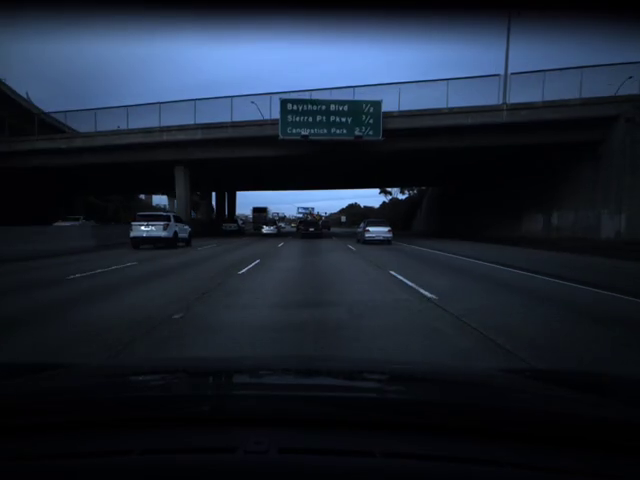
\includegraphics[width=.35\columnwidth]{./imgs/frame2_original.png}} \hspace{0.1cm}
  \subfloat[Frame after initial down sampling]{\label{figur:2}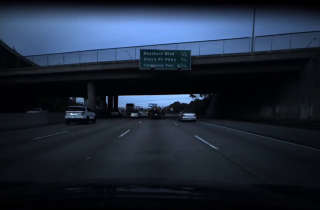
\includegraphics[width=.35\columnwidth]{./imgs/frame2_cut_sampled.png}}\\
  \subfloat[Optical Flow field, already down sampled]{\label{figur:3}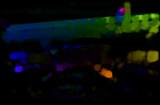
\includegraphics[width=0.6\columnwidth]{./imgs/frame2_flow_field.png}}
  \label{figur}\caption{Preprocessing of the video frames.}
\end{figure}

%\begin{figure}[h!]
%\centering
%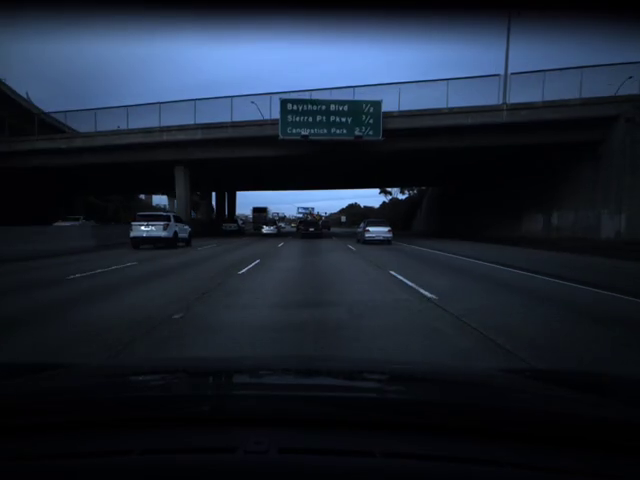
\includegraphics[width=0.7\columnwidth]{./imgs/frame2_original.png}
%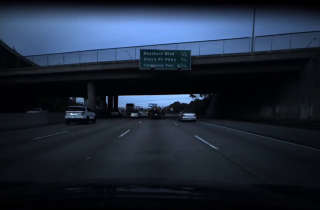
\includegraphics[width=0.7\columnwidth]{./imgs/frame2_cut_sampled.png}
%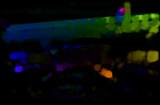
\includegraphics[width=0.7\columnwidth]{./imgs/frame2_flow_field.png}
%\end{figure}
Explain, how we show the optical flow.

\section{Method selection and architecture}

\section{Results and comparison}

\section{Further work}
%
%
%
%{\BibTeX} does not work by magic. It doesn't get the bibliographic
%data from thin air but from .bib files. If you use {\BibTeX} to produce a
%bibliography you must send the .bib files. 
%
%{\LaTeX} can't read your mind. If you assign the same label to a
%subsubsection and a table, you might find that Table I has been cross
%referenced as Table IV-B3. 
%
%{\LaTeX} does not have precognitive abilities. If you put a
%\verb|\label| command before the command that updates the counter it's
%supposed to be using, the label will pick up the last counter to be
%cross referenced instead. In particular, a \verb|\label| command
%should not go before the caption of a figure or a table.
%
%Do not use \verb|\nonumber| inside the \verb|{array}| environment. It
%will not stop equation numbers inside \verb|{array}| (there won't be
%any anyway) and it might stop a wanted equation number in the
%surrounding equation.
%
%\subsection{Some Common Mistakes}\label{SCM}
%\begin{itemize}
%\item The word ``data'' is plural, not singular.
%\item The subscript for the permeability of vacuum $\mu_{0}$, and other common scientific constants, is zero with subscript formatting, not a lowercase letter ``o''.
%\item In American English, commas, semicolons, periods, question and exclamation marks are located within quotation marks only when a complete thought or name is cited, such as a title or full quotation. When quotation marks are used, instead of a bold or italic typeface, to highlight a word or phrase, punctuation should appear outside of the quotation marks. A parenthetical phrase or statement at the end of a sentence is punctuated outside of the closing parenthesis (like this). (A parenthetical sentence is punctuated within the parentheses.)
%\item A graph within a graph is an ``inset'', not an ``insert''. The word alternatively is preferred to the word ``alternately'' (unless you really mean something that alternates).
%\item Do not use the word ``essentially'' to mean ``approximately'' or ``effectively''.
%\item In your paper title, if the words ``that uses'' can accurately replace the word ``using'', capitalize the ``u''; if not, keep using lower-cased.
%\item Be aware of the different meanings of the homophones ``affect'' and ``effect'', ``complement'' and ``compliment'', ``discreet'' and ``discrete'', ``principal'' and ``principle''.
%\item Do not confuse ``imply'' and ``infer''.
%\item The prefix ``non'' is not a word; it should be joined to the word it modifies, usually without a hyphen.
%\item There is no period after the ``et'' in the Latin abbreviation ``et al.''.
%\item The abbreviation ``i.e.'' means ``that is'', and the abbreviation ``e.g.'' means ``for example''.
%\end{itemize}
%An excellent style manual for science writers is \cite{b7}.
%
%\subsection{Authors and Affiliations}
%\textbf{The class file is designed for, but not limited to, six authors.} A 
%minimum of one author is required for all conference articles. Author names 
%should be listed starting from left to right and then moving down to the 
%next line. This is the author sequence that will be used in future citations 
%and by indexing services. Names should not be listed in columns nor group by 
%affiliation. Please keep your affiliations as succinct as possible (for 
%example, do not differentiate among departments of the same organization).
%
%\subsection{Identify the Headings}
%Headings, or heads, are organizational devices that guide the reader through 
%your paper. There are two types: component heads and text heads.
%
%Component heads identify the different components of your paper and are not 
%topically subordinate to each other. Examples include Acknowledgments and 
%References and, for these, the correct style to use is ``Heading 5''. Use 
%``figure caption'' for your Figure captions, and ``table head'' for your 
%table title. Run-in heads, such as ``Abstract'', will require you to apply a 
%style (in this case, italic) in addition to the style provided by the drop 
%down menu to differentiate the head from the text.
%
%Text heads organize the topics on a relational, hierarchical basis. For 
%example, the paper title is the primary text head because all subsequent 
%material relates and elaborates on this one topic. If there are two or more 
%sub-topics, the next level head (uppercase Roman numerals) should be used 
%and, conversely, if there are not at least two sub-topics, then no subheads 
%should be introduced.
%
%\subsection{Figures and Tables}
%\paragraph{Positioning Figures and Tables} Place figures and tables at the top and 
%bottom of columns. Avoid placing them in the middle of columns. Large 
%figures and tables may span across both columns. Figure captions should be 
%below the figures; table heads should appear above the tables. Insert 
%figures and tables after they are cited in the text. Use the abbreviation 
%``Fig.~\ref{fig}'', even at the beginning of a sentence.
%
%\begin{table}[htbp]
%\caption{Table Type Styles}
%\begin{center}
%\begin{tabular}{|c|c|c|c|}
%\hline
%\textbf{Table}&\multicolumn{3}{|c|}{\textbf{Table Column Head}} \\
%\cline{2-4} 
%\textbf{Head} & \textbf{\textit{Table column subhead}}& \textbf{\textit{Subhead}}& \textbf{\textit{Subhead}} \\
%\hline
%copy& More table copy$^{\mathrm{a}}$& &  \\
%\hline
%\multicolumn{4}{l}{$^{\mathrm{a}}$Sample of a Table footnote.}
%\end{tabular}
%\label{tab1}
%\end{center}
%\end{table}



%Figure Labels: Use 8 point Times New Roman for Figure labels. Use words 
%rather than symbols or abbreviations when writing Figure axis labels to 
%avoid confusing the reader. As an example, write the quantity 
%``Magnetization'', or ``Magnetization, M'', not just ``M''. If including 
%units in the label, present them within parentheses. Do not label axes only 
%with units. In the example, write ``Magnetization (A/m)'' or ``Magnetization 
%\{A[m(1)]\}'', not just ``A/m''. Do not label axes with a ratio of 
%quantities and units. For example, write ``Temperature (K)'', not 
%``Temperature/K''.

\section*{Acknowledgment}

The preferred spelling of the word ``acknowledgment'' in America is without 
an ``e'' after the ``g''. Avoid the stilted expression ``one of us (R. B. 
G.) thanks $\ldots$''. Instead, try ``R. B. G. thanks$\ldots$''. Put sponsor 
acknowledgments in the unnumbered footnote on the first page.



\begin{thebibliography}{00}
\bibitem{b1} G. Eason, B. Noble, and I. N. Sneddon, ``On certain integrals of Lipschitz-Hankel type involving products of Bessel functions,'' Phil. Trans. Roy. Soc. London, vol. A247, pp. 529--551, April 1955.
\bibitem{b2} J. Clerk Maxwell, A Treatise on Electricity and Magnetism, 3rd ed., vol. 2. Oxford: Clarendon, 1892, pp.68--73.
\bibitem{b3} I. S. Jacobs and C. P. Bean, ``Fine particles, thin films and exchange anisotropy,'' in Magnetism, vol. III, G. T. Rado and H. Suhl, Eds. New York: Academic, 1963, pp. 271--350.
\bibitem{b4} K. Elissa, ``Title of paper if known,'' unpublished.
\bibitem{b5} R. Nicole, ``Title of paper with only first word capitalized,'' J. Name Stand. Abbrev., in press.
\bibitem{b6} Y. Yorozu, M. Hirano, K. Oka, and Y. Tagawa, ``Electron spectroscopy studies on magneto-optical media and plastic substrate interface,'' IEEE Transl. J. Magn. Japan, vol. 2, pp. 740--741, August 1987 [Digests 9th Annual Conf. Magnetics Japan, p. 301, 1982].
\bibitem{b7} M. Young, The Technical Writer's Handbook. Mill Valley, CA: University Science, 1989.
\end{thebibliography}


\end{document}
